\section{Multiphonon response}\label{sec:11.3}

At $q_{\mathrm{BZ}} = \SI{2.25}{keV}$ the long-wavelength phonons of \cref{sec:11.1} stop describing the response, and at about 90 to \SI{140}{keV} the free recoil of \cref{sec:11.4} becomes valid (by the two onset criteria compared there). Between these two momenta, a silicon nucleus that takes up the momentum $\vect{q}$ leaves behind zero, one, two or a dozen phonons. Dark matter between about 0.4 and \SI{26}{MeV} transfers its largest momenta, $2\mchi v_{\mathrm{max}}$, inside this window. \Cref{sec:5.6} computed the response of one nucleus as if the others were not there: the phonon number is Poisson distributed with mean $2W_\kappa(\vect{q})$, and the spectrum of each term follows from the density of states. A crystal adds the pairs of different nuclei, whose interference produced the conservation of crystal momentum in the one-phonon response of \cref{sec:11.1}. How much of that interference survives when two or more phonons share the momentum, and when may a calculation drop it? The incoherent approximation of the literature drops the pairs. It is exact on average far above the zone for a lattice without a basis, and in silicon its phonon-number weights are good to \SI{10}{\percent} above about \SI{6.6}{keV}.

\subsection{The response at all phonon orders}

We keep the coupling of \cref{sec:11.1}, a potential $\tilde V_N(\vect{q})$ that sees each nucleus of species $\kappa$ with a weight $c_\kappa$, so that the dark matter couples to the operator $\sum_\kappa c_\kappa n_\kappa(\vect{q})$. For equal couplings to protons and neutrons $c_\kappa = A_\kappa$, the nucleon number. The results below hold for any coupling that multiplies the density of each species by a real number, the coefficient $c_1^{(\kappa)}$ of \cref{sec:8.4}, and in particular for the rigid-ion charge $Z_\kappa$. We keep writing $S_A$ for the response, as in \cref{sec:11.1}, and \cref{eq:8.2-spectrum} with one row turns it into a rate. The nuclei sit at $\vect{X}_{\vect{R}\kappa} = \vect{R} + \vect{\tau}_\kappa + \vect{u}_{\vect{R}\kappa}$, and $n_\kappa(\vect{q}) = \sum_{\vect{R}}\ee^{\ii\vect{q}\cdot\vect{X}_{\vect{R}\kappa}}$. The correlation form of \cref{eq:4.2-Sab} then contains, for every pair of nuclei, the average $\langle\ee^{-\ii\vect{q}\cdot\vect{X}_{\vect{R}\kappa}(t)}\ee^{\ii\vect{q}\cdot\vect{X}_{\vect{R}'\kappa'}(0)}\rangle$. The static positions give a phase, and the displacements give the generating formula of a pair, \cref{eq:D.15-gen}. The average depends only on the separation $\Delta\vect{R} = \vect{R} - \vect{R}'$ of the cells, because the eigenvectors carry the cell phase $\ee^{\ii\vect{Q}\cdot\vect{R}}$ (\cref{eq:5.3-u}) and the thermal state is invariant under lattice translations. The sum over $\vect{R}'$ then gives a factor $N$, and with the volume $\Vol = N\Omega$ we find
\begin{keyresult}[Harmonic nuclear response at all phonon orders]
\begin{equation}
  S_A(\vect{q},\omega) = \frac1\Omega\sum_{\Delta\vect{R},\kappa,\kappa'}c_\kappa c_{\kappa'}\,\ee^{-\ii\vect{q}\cdot\Delta\vect{R}_{\kappa\kappa'}}\,\ee^{-W_\kappa(\vect{q}) - W_{\kappa'}(\vect{q})}\int_{-\infty}^{\infty}\dd t\;\ee^{\ii\omega t}\,\ee^{\vect{q}\cdot\mathcal{C}_{\kappa\kappa'}(\Delta\vect{R},t)\cdot\vect{q}} ,
  \label{eq:11.3-exact}
\end{equation}
with $\Delta\vect{R}_{\kappa\kappa'} = \Delta\vect{R} + \vect{\tau}_\kappa - \vect{\tau}_{\kappa'}$ the vector from nucleus $\kappa'$ in the cell at the origin to nucleus $\kappa$ in the cell $\Delta\vect{R}$, the Debye--Waller exponents of \cref{eq:5.6-W} and the displacement correlation of \cref{eq:5.6-C}. \Cref{eq:11.3-exact} holds for a harmonic crystal in thermal equilibrium at any temperature.
\end{keyresult}
\noindent This response is the classical starting point of neutron scattering from crystals~\cite[App.~N]{ashcroft1976solid}, written for a coupling that differs from species to species. Every quantity in it was computed in \cref{sec:5.6} from the force constants. The sum over pairs is new. Its terms with $\Delta\vect{R}_{\kappa\kappa'} = 0$, one nucleus scattering at both times, form the \emph{self part}, which is \cref{eq:5.6-multi} weighted by $c_\kappa^2$ and summed over the basis. All other terms form the \emph{distinct part}. Each distinct term carries the phase $\ee^{-\ii\vect{q}\cdot\Delta\vect{R}_{\kappa\kappa'}}$, and its size is set by how strongly the displacements of two nuclei a distance $|\Delta\vect{R}_{\kappa\kappa'}|$ apart are correlated.

Expanding the last exponential in powers of $\vect{q}\cdot\mathcal{C}_{\kappa\kappa'}\cdot\vect{q}$ sorts the response by the number $n$ of phonons, $S_A = \sum_nS^{(n)}_A$, as in \cref{sec:5.6}. The term $n = 0$ is time independent. Its sum over $\Delta\vect{R}$ vanishes unless $\vect{q}$ is a reciprocal-lattice vector, and the term is the Bragg peak, $\propto\delta(\omega)\sum_{\vect{G}}\delta^3(\vect{q} - \vect{G})$. The Bragg peak deposits no energy and occupies a set of zero measure in $\vect{q}$, so it never contributes to a rate. For $n \ge 1$ each factor $\vect{q}\cdot\mathcal{C}_{\kappa\kappa'}\cdot\vect{q}$ is a sum over phonons $\vect{Q}\nu$ with the phase $\ee^{\ii\vect{Q}\cdot\Delta\vect{R}}$, and the sum over $\Delta\vect{R}$ against $\ee^{-\ii\vect{q}\cdot\Delta\vect{R}}$ forces the phonon wavevectors to add up to $\vect{q}$ up to a reciprocal-lattice vector. Each phonon $i$ is created ($s_i = +1$) or absorbed ($s_i = -1$), and after the time integral (\cref{app:D.31})
\begin{keyresult}[The $n$-phonon term]
\begin{equation}
  \begin{aligned}
  S^{(n)}_A(\vect{q},\omega) = \frac{2\pi}{\Omega}\,\frac{1}{n!}\sum_{\{\nu_i,s_i\}}\Bigl\langle\,&\prod_{i=1}^{n}\frac{n_{\vect{Q}_i\nu_i} + \frac12(1 + s_i)}{2\omega_{\vect{Q}_i\nu_i}}\;\delta\Bigl(\omega - \sum_is_i\omega_{\vect{Q}_i\nu_i}\Bigr) \\
  &\times\Bigl|\sum_\kappa c_\kappa\,\ee^{-W_\kappa}\,\ee^{\ii\vect{q}\cdot\vect{\tau}_\kappa}\,\frac{\prod_i\vect{q}\cdot\vect{e}^{s_i}_{\kappa\nu_i}(\vect{Q}_i)}{M_\kappa^{n/2}}\Bigr|^2\Bigr\rangle ,
  \end{aligned}
  \label{eq:11.3-Sn}
\end{equation}
with $\vect{e}^{+} = \vect{e}^*$ for a created and $\vect{e}^{-} = \vect{e}$ for an absorbed phonon, $\vect{q}$ unreduced in the phase $\ee^{\ii\vect{q}\cdot\vect{\tau}_\kappa}$, and the brackets the average $N^{-(n-1)}\sum$ over $\vect{Q}_1, \ldots, \vect{Q}_{n-1}$ in the zone, with $\vect{Q}_n$ fixed by $\sum_is_i\vect{Q}_i = \vect{q} - \vect{G}$.
\end{keyresult}
\noindent At $n = 1$ the brackets are empty, $\vect{Q}_1 = \vect{q} - \vect{G}$ for emission, and \cref{eq:11.3-Sn} is the one-phonon response \cref{eq:11.1-S1}. For every $n$ the crystal momentum is conserved, and the response at fixed $\vect{q}$ is a convolution over the zone of $n$ branches. \Cref{eq:11.3-Sn} is the full harmonic answer, and also an expensive one: at $n = 2$ the sum runs over one wavevector of the zone for each $\vect{q}$, at $n = 3$ over two.

On the truncation label of \cref{sec:8.5}, \cref{eq:11.3-exact} is at $n_A = 0$ and $n_B = 0$, with every thermal order kept through the factors $n_{\vect{Q}\nu}$, and with $\mathcal{K}$ = multiphonon, all orders. In a detector at \SI{10}{mK} only the terms with every $s_i = +1$ survive, at $n_T = 0$.

In neutron scattering, ``incoherent'' refers to the random variation of the coupling from site to site, between isotopes or nuclear spin states. For a nucleon-number coupling in natural silicon the variance of $A_\kappa$ is 0.159, $2.0\times10^{-4}$ of $\langle A_\kappa\rangle^2 = 790.1$, and negligible; the isotopes act instead through their masses (\cref{sec:11.6}). Here ``incoherent'' means the approximation that keeps only the self part.

The quantities in \cref{eq:11.3-exact,eq:11.3-Sn} come from one harmonic calculation per material: DFPT force constants, interpolated to a fine grid of wavevectors, give the frequencies and polarization vectors, from which the exponents $W_\kappa$, the correlations $\mathcal{C}_{\kappa\kappa'}$ and the zone sums follow at negligible cost (\cref{sec:5.4,app:E.17}).

\subsection{The incoherent approximation}

At momentum transfers far above the zone, the phase $\ee^{-\ii\vect{q}\cdot\Delta\vect{R}_{\kappa\kappa'}}$ of a distinct term turns through many radians when $\vect{q}$ changes by a fraction of $q_{\mathrm{BZ}}$. The other factors of the distinct term, a polynomial in $\vect{q}$ times the Debye--Waller factors, barely change. Any rate integrates over $\vect{q}$, and the distinct terms then average away, leaving the self part, which treats each nucleus as an independent oscillator in the potential well of its neighbors:
\begin{equation}
  S_A(\vect{q},\omega) \approx S^{\mathrm{inc}}_A(\vect{q},\omega) = \frac{2\pi}{\Omega}\sum_\kappa c_\kappa^2\,\ee^{-2W_\kappa(\vect{q})}\sum_{n=0}^{\infty}\frac{[2W_\kappa(\vect{q})]^n}{n!}\,P^\kappa_n(\hat{\vect{q}},\omega) .
  \label{eq:11.3-inc}
\end{equation}
Here $P^\kappa_1(\hat{\vect{q}},\omega)$ is the single-phonon distribution of \cref{sec:5.6} for nucleus $\kappa$: the density of states projected on the direction of $\vect{q}$, $N^{-1}\sum_{\vect{Q}\nu}|\hat{\vect{q}}\cdot\vect{e}_{\kappa\nu}(\vect{Q})|^2\delta(\omega - \omega_{\vect{Q}\nu})$, times $[n_{\mathrm{B}}(\omega) + 1]/\omega$, normalized to one. $P^\kappa_n$ is the $n$-fold convolution of $P^\kappa_1$. On a site of cubic symmetry the projected density of states is a third of the atom-projected one, $g_{\mathrm{ph},\kappa}(\omega)/3$, independent of $\hat{\vect{q}}$, and \cref{eq:11.3-inc} is \cref{eq:5.6-multi} summed over the basis.

The incoherent approximation keeps the self part exactly, so it inherits two exact properties from \cref{sec:5.6}: the phonon number is Poisson distributed, and the first moment of the response, $\int\dd\omega\,\omega S_A$, is $(2\pi/\Omega)\sum_\kappa c_\kappa^2E_R$ with $E_R = q^2/2M_\kappa$. The distinct part adds weight but no energy. Every distinct term has zero first moment in $\omega$, at every order $n$, because its time derivative at $t = 0$ contains $\partial_t\mathcal{C}_{\kappa\kappa'}(\Delta\vect{R},0)$, which the completeness of the polarization vectors makes proportional to $\delta_{\kappa\kappa'}\delta_{\Delta\vect{R},\vect{0}}$ (\cref{app:D.31}). The first moment of the $n$-phonon term is therefore the first moment of its self part, and for one species
\begin{equation}
  \frac{\int\dd\omega\;\omega\,S^{(n)}_A(\vect{q},\omega)}{\int\dd\omega\;\omega\,S_A(\vect{q},\omega)} = \ee^{-2W_\kappa}\,\frac{(2W_\kappa)^{n-1}}{(n-1)!} ,
  \label{eq:11.3-fsum}
\end{equation}
at every $\vect{q}$ and temperature, coherent terms included. A calculation that stops at order $N$ misses the fraction $\sum_{n \ge N}p^{\mathrm{ph}}_n$ of the recoil energy, the Poisson tail of the weights \cref{eq:5.6-poisson}; with several species the fractions are averaged with the weights $c_\kappa^2/M_\kappa$. At \SI{50}{keV} in silicon, where $2W_\kappa = 1.57$, the orders above two carry \SI{47}{\percent} of the energy deposited, and a two-phonon calculation misses that share.

The tail matters most for a threshold above the phonon band. Since $P^\kappa_n$ vanishes above $n\,\omega_{\mathrm{max}}$, with $\omega_{\mathrm{max}}$ the highest phonon energy, an energy deposit above $E$ needs at least $\lceil E/\omega_{\mathrm{max}}\rceil$ phonons, and in the incoherent approximation at $T = 0$ its probability is at most the Poisson tail $\sum_{n \ge \lceil E/\omega_{\mathrm{max}}\rceil}p^{\mathrm{ph}}_n$. A free nucleus deposits exactly $E_R$.

\begin{workedexample}{The Poisson tail above three Debye energies}\label{we:11-tail}
Take silicon at $T = 0$ and a threshold $E = 3\omega_{\mathrm{D}} = \SI{166.8}{meV}$, with $\omega_{\mathrm{D}} = \SI{55.6}{meV}$ from \cref{we:5-dw}. The computed density of states of \cref{sec:5.2} ends at $\omega_{\mathrm{max}} = \SI{63.7}{meV}$ (the zone-center optical phonon measured by neutron scattering at room temperature is \SI{64.1}{meV}, \cref{sec:5.2}), so two phonons reach at most \SI{127}{meV} and a deposit above $E$ needs three or more. Of the three-phonon spectrum $P_3$, \SI{1.4}{\percent} lies above $E$; of $P_4$, $P_5$ and $P_6$, 11, 35 and \SI{62}{\percent}. With $2W_\kappa = q^2\langle u_x^2\rangle$ and $\langle u_x^2\rangle = \SI{2.45e-3}{\angstrom^2}$, the probability of a deposit above $E$ is $\sum_np^{\mathrm{ph}}_n\int_E^\infty P_n$:

\emph{$q = \SI{10}{keV}$.} $E_R = \SI{1.91}{meV}$ and $2W_\kappa = 0.063$. The probability is \num{6.1e-7}, almost all of it from three phonons; the Poisson bound $\sum_{n\ge3}p^{\mathrm{ph}}_n = \num{4.0e-5}$ is 65 times larger, because a three-phonon deposit rarely reaches the top of its band.

\emph{$q = \SI{30}{keV}$.} $E_R = \SI{17.2}{meV}$ and $2W_\kappa = 0.566$. The probability is \num{6.2e-4}, from three, four and five phonons in the proportion 0.38 : 0.43 : 0.16; the bound is \num{2.0e-2}.

\emph{$q = \SI{50}{keV}$.} $E_R = \SI{47.8}{meV}$, a third of the threshold, and $2W_\kappa = 1.57$. The probability is \num{1.7e-2}, against the bound 0.21. Four and five phonons contribute most.

A free silicon nucleus deposits \SI{166.8}{meV} only for $q \ge (2M_\kappa E)^{1/2} = \SI{93.4}{keV}$. A particle much lighter than the nucleus transfers at most $2\mchi v_{\mathrm{max}}$, so the free-recoil picture needs $\mchi \ge \SI{17.6}{MeV}$ for this threshold. Dark matter of \SI{10}{MeV} reaches $q = \SI{53}{keV}$, and already at \SI{50}{keV} the bound lattice deposits more than $3\omega_{\mathrm{D}}$ in \SI{1.7}{\percent} of the scatterings.
\end{workedexample}

\Cref{app:D.31} finds the range of the incoherent approximation by averaging $\vect{q}$ over a small cell of reciprocal space, the size of the zone, around a given $\vect{q}$. The phase of a distinct term averages to $j_{\mathrm{BZ}}(\Delta\vect{R}_{\kappa\kappa'}) = (\Omega/(2\pi)^3)\int_{\mathrm{BZ}}\dd^3p\,\ee^{-\ii\vect{p}\cdot\Delta\vect{R}_{\kappa\kappa'}}$, which vanishes for every lattice vector except zero, while the slowly varying factors change across the cell by a relative amount of order $n\,q_{\mathrm{BZ}}/q$. For a lattice with one atom per cell every distinct term joins two nuclei of the same sublattice, and the incoherent response is the average of the exact one over a zone-sized cell, up to corrections of relative order $nq_{\mathrm{BZ}}/q$. With a basis the pairs on different sublattices are not separated by lattice vectors, and they survive the average: in silicon each of the four bonds keeps a weight $j_{\mathrm{BZ}} \approx 0.44$ in a spherical zone. The distinct terms of the bonds decay because the correlation of two displacements falls with distance. The average over the directions of $\vect{q}$, as in the rate of a crystal of random orientation, reduces each of them further by a spherical Bessel function of $q|\Delta\vect{R}_{\kappa\kappa'}|$. The incoherent approximation therefore needs $q \gg \max(n, 2W_\kappa)\,q_{\mathrm{BZ}}$, and for a crystal with a basis the size of the surviving distinct terms has to be computed.

\begin{limitbox}[Multiphonon incoherent approximation][lim:11.3a]
Above the zone, the nuclear response is the sum of independent atomic responses, each a Poisson series in the phonon number, $S \approx (2\pi/\Omega)\sum_\kappa c_\kappa^2\ee^{-2W_\kappa}\sum_n[(2W_\kappa)^n/n!]P^\kappa_n(\omega)$, with $P^\kappa_n$ the $n$-fold convolution of the single-phonon distribution~\cite[Eqs.~(15), (36)]{campbelldeem2022dark}.
\par\smallskip
{\centering
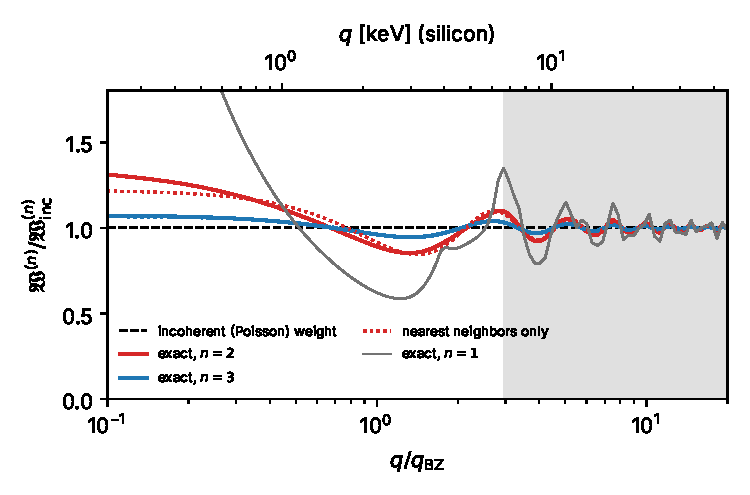
\includegraphics[width=\linewidth]{figures/ch11/limit11_3a.pdf}
\captionof{figure}{The exact $\omega$-integrated $n$-phonon weight of silicon at $T = 0$, \cref{eq:11.3-weight}, divided by its incoherent value, the Poisson weight of \cref{eq:11.3-inc} (dashed, one), averaged over the directions of $\vect{q}$, against $q/q_{\mathrm{BZ}}$, with $q_{\mathrm{BZ}} = \SI{2.25}{keV}$. For one species the couplings and the Debye--Waller factors cancel in the ratio, which is $1 + \delta^{\mathrm{coh}}_n(q)$ for any coupling of the form $\sum_\kappa c_\kappa n_\kappa$. Displacement correlations from the PBE force constants of \cref{sec:5.2} on a $48^3$ grid, pair sum to \SI{40}{\angstrom}, direction average exact. Solid: two (red) and three (blue) phonons. Dotted: the nearest-neighbor pairs alone, the leading correction. Thin gray: one phonon, which must be summed in reciprocal space. Gray band: $q \ge 2.95\,q_{\mathrm{BZ}} = \SI{6.6}{keV}$, where the two- and three-phonon weights stay within \SI{10}{\percent} of the incoherent ones. The three-phonon weight does so at every $q$, the one-phonon weight only above $7.9\,q_{\mathrm{BZ}}$.}\label{fig:11-limit-3a}
\par}
\smallskip
Below about three times the zone momentum the two-phonon weight differs from the Poisson weight by up to \SI{35}{\percent}, and pointwise in $\omega$ the incoherent spectrum misses the momentum conservation of the phonon pair even far above the zone.
\end{limitbox}

At small $q$ the phases are irrelevant, and every pair adds with the square of its correlation. The coherent two-phonon weight then exceeds the incoherent one by \SI{35}{\percent}, mostly from the four bonds, along which the longitudinal displacements of neighbors are correlated with a coefficient of 0.44 (a dynamical number, distinct from the geometric weight $j_{\mathrm{BZ}} \approx 0.44$ above, to which it is close by coincidence). Near $q_{\mathrm{BZ}}$ the bond phases turn the sign of this correction, and from about $3\,q_{\mathrm{BZ}}$ the correction oscillates with the period of the bond length and decays: $\delta^{\mathrm{coh}}_2 = -0.079$, $+0.014$, $-0.018$ and $-0.025$ at 2, 5, 10 and \SI{20}{keV}. The nearest-neighbor pairs alone account for 0.21 of the 0.35 at small $q$, and above about $2\,q_{\mathrm{BZ}}$ they follow the full curve within \SI{1}{\percent} of the weight. The three-phonon correction is smaller everywhere, since it carries the cube of a correlation coefficient below one: $-0.027$, $+0.016$, $-0.006$ and $-0.012$ at the same momentum transfers. The one-phonon term is the exception: it is sharp in $\omega$ at fixed $\vect{q}$, its pair sum does not converge absolutely, and its $\omega$-integrated weight approaches the incoherent value slowly, within \SI{10}{\percent} above about \SI{18}{keV}. Near each reciprocal-lattice vector the soft acoustic phonons enhance the one-phonon weight. Above $q_{\mathrm{BZ}}$, where \cref{eq:11.1-Sac} no longer holds, the one-phonon term is computed from \cref{eq:11.1-S1} with all branches and Umklapp terms, and its weight grows on average as $q^2\ee^{-2W_\kappa}$, the incoherent form, up to these corrections.

\Cref{fig:11-mph} shows the three parts of the silicon response at $q = \SI{10}{keV}$, the momentum transfer at which \cref{sec:8.5} placed the end of the one-phonon regime. One phonon carries a weight of 0.058 per nucleus, two phonons \num{1.8e-3} and three or more \num{4.0e-5}, close to the Poisson weights $2W_\kappa\ee^{-2W_\kappa} = 0.059$, $(2W_\kappa)^2\ee^{-2W_\kappa}/2 = \num{1.9e-3}$ and the rest. The exact one-phonon spectrum, averaged over directions, follows the projected density of states. The exact two-phonon spectrum follows the self-convolution of the single-phonon distribution within \SI{17}{\percent} in every bin of \SI{1}{meV} between 22 and \SI{120}{meV}, where the spectrum exceeds a tenth of its maximum; toward the edges of the band the ratio of the exact to the incoherent spectrum falls to about one half.

\begin{figure}[tbp]
  \centering
  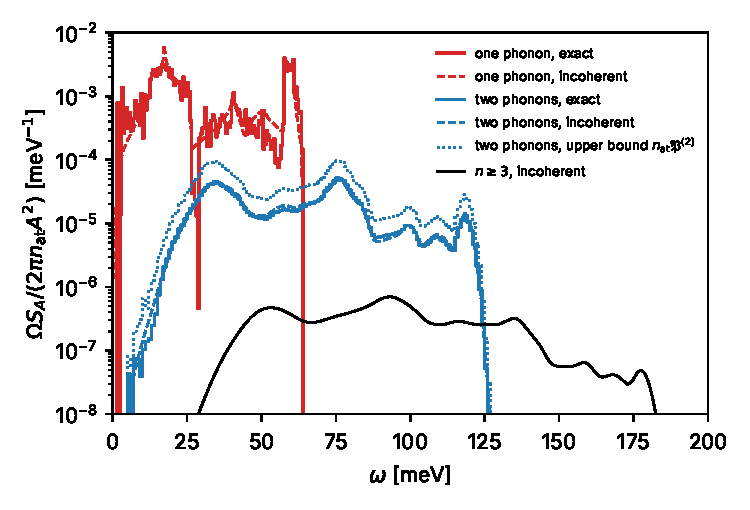
\includegraphics[width=\linewidth]{figures/ch11/fig11_3.pdf}
  \caption{Nuclear response of silicon at $|\vect{q}| = \SI{10}{keV}$ and $T = 0$, per nucleus, $\Omega S_A/(2\pi n_{\mathrm{at}}A^2)$, averaged over the directions of $\vect{q}$, split by the number of phonons; the elastic weight $\ee^{-2W_\kappa} = 0.939$ at $\omega = 0$ is not shown. Red: one phonon, exact (\cref{eq:11.1-S1}, all six branches, histogram of 0.5-meV bins) and incoherent (dashed). Blue: two phonons, exact (\cref{eq:11.3-Sn}, 1-meV bins), incoherent (dashed) and the upper end $n_{\mathrm{at}}\mathfrak{P}^{(2)}$ of the certified band \cref{eq:11.3-band} (dotted). Black: three or more phonons, incoherent. Phonons from the PBE force constants of \cref{sec:5.2}; incoherent parts from the density of states of the same force constants, with $\langle u_x^2\rangle = \SI{2.45e-3}{\angstrom^2}$. The exact two-phonon response is averaged over 240 wavevectors with $|\vect{q}|$ within \SI{1}{\percent} of \SI{10}{keV} on a $24^3$ grid commensurate with the zone, each rescaled to \SI{10}{keV} by $(10\,\mathrm{keV}/|\vect{q}|)^4$.}
  \label{fig:11-mph}
\end{figure}

\subsection{Exact phonon-order weights}

Integration over $\omega$ reduces the time integral of \cref{eq:11.3-exact} to the integrand at $t = 0$, and the $n$-phonon term becomes a sum over pairs of a static quantity. At $t = 0$ the two terms of \cref{eq:5.6-C} combine into $2n_{\vect{Q}\nu} + 1$, and the displacement correlation becomes the static correlation tensor
\begin{equation}
  B_{\kappa\kappa'}(\Delta\vect{R}) = \mathcal{C}_{\kappa\kappa'}(\Delta\vect{R},0) = \frac1N\sum_{\vect{Q}\nu}(2n_{\vect{Q}\nu} + 1)\,\frac{\vect{e}_{\kappa\nu}(\vect{Q})\,\vect{e}_{\kappa'\nu}(\vect{Q})^\dagger\,\ee^{\ii\vect{Q}\cdot\Delta\vect{R}}}{2\omega_{\vect{Q}\nu}\sqrt{M_\kappa M_{\kappa'}}} ,
  \label{eq:11.3-Bkk}
\end{equation}
whose on-site value $B_{\kappa\kappa}(\vect{0})$ is the displacement tensor $B_\kappa$ of \cref{eq:5.3-B}. Off site it measures how the displacements of two nuclei move together: $\langle u^\alpha_{\Delta\vect{R}\kappa}u^\beta_{\vect{0}\kappa'}\rangle$.
\begin{keyresult}[Exact $n$-phonon weight]
The $\omega$-integrated $n$-phonon response per cell is
\begin{equation}
  \mathfrak{W}^{(n)}(\vect{q}) = \Omega\int\frac{\dd\omega}{2\pi}\,S^{(n)}_A(\vect{q},\omega) = \frac{1}{n!}\sum_{\Delta\vect{R},\kappa,\kappa'}c_\kappa c_{\kappa'}\,\ee^{-\ii\vect{q}\cdot\Delta\vect{R}_{\kappa\kappa'}}\,\ee^{-W_\kappa - W_{\kappa'}}\,\bigl[\vect{q}\cdot B_{\kappa\kappa'}(\Delta\vect{R})\cdot\vect{q}\bigr]^n .
  \label{eq:11.3-weight}
\end{equation}
Its self terms are the incoherent weight $\mathfrak{W}^{(n)}_{\mathrm{inc}} = \sum_\kappa c_\kappa^2\,\ee^{-2W_\kappa}(2W_\kappa)^n/n!$, and $\delta^{\mathrm{coh}}_n(\vect{q}) = \mathfrak{W}^{(n)}/\mathfrak{W}^{(n)}_{\mathrm{inc}} - 1$ is the exact correction to the incoherent approximation for any energy window that contains the whole $n$-phonon band.
\end{keyresult}
\noindent A rate code applies this exact correction as a factor $1 + \delta^{\mathrm{coh}}_n$ per phonon order. At $T = 0$ the acoustic modes near $\mathrm{\Gamma}$ make $B_{\kappa\kappa'}(\Delta\vect{R})$ fall as $|\Delta\vect{R}|^{-2}$ at large distances (\cref{app:D.31}). Its square falls as $|\Delta\vect{R}|^{-4}$, faster than the number of pairs grows, and the sum converges absolutely for $n \ge 2$. For $n = 1$ the sum does not converge absolutely, and the one-phonon term is summed in reciprocal space, where it is \cref{eq:11.1-S1}. At $T > 0$ the thermal occupation of the same modes makes $B_{\kappa\kappa'}$ fall only as $T/|\Delta\vect{R}|$, and the two-phonon sum diverges; the subsection on thermal diffuse scattering resums it.

In silicon at $T = 0$ the correlation is short ranged in practice. With the force constants of \cref{sec:5.2} on a $48^3$ grid of wavevectors, the on-site value is $\langle u_x^2\rangle = \SI{2.45e-3}{\angstrom^2}$, as in \cref{we:5-dw}. The sum of \cref{eq:11.3-weight} to \SI{40}{\angstrom} takes seconds for any $\vect{q}$, and changes by less than $2\times10^{-3}$ beyond \SI{30}{\angstrom}. This sum produced the curves of \cref{fig:11-limit-3a}.

The $\omega$-integrated weight leaves open how the coherent correction is distributed in $\omega$. A pointwise statement follows from the structure of \cref{eq:11.3-Sn}, in which the coherent sum over the basis appears inside a squared modulus. By the Cauchy--Schwarz inequality, $|\sum_\kappa a_\kappa|^2 \le n_{\mathrm{at}}\sum_\kappa|a_\kappa|^2$ for the $n_{\mathrm{at}}$ nuclei of a cell, term by term in the sum over phonons. The \emph{momentum-resolved self density} $\mathfrak{P}^{(n)}(\vect{q},\omega)$ is \cref{eq:11.3-Sn} with the squared modulus replaced by the sum of the squared amplitudes of the single nuclei: the response of independent nuclei whose $n$ phonons must still add up to the crystal momentum $\vect{q}$. For silicon, $n_{\mathrm{at}} = 2$, and with $a_1$, $a_2$ the amplitudes of the two nuclei of a cell for one set of phonons, $|a_1 + a_2|^2 = 2(|a_1|^2 + |a_2|^2) - |a_1 - a_2|^2 \le 2(|a_1|^2 + |a_2|^2)$, with equality when the two nuclei move in phase.
\begin{keyresult}[Certified band]
At every $\vect{q}$, $\omega$ and $n$,
\begin{equation}
  \begin{gathered}
  0 \le S^{(n)}_A(\vect{q},\omega) \le n_{\mathrm{at}}\,\mathfrak{P}^{(n)}(\vect{q},\omega) , \\
  \frac{\Omega}{(2\pi)^3}\int_{\mathrm{BZ}}\dd^3p\;\mathfrak{P}^{(n)}(\vect{q} + \vect{p},\omega)\Big|_{\text{vertex at }\vect{q}} = S^{\mathrm{inc},(n)}_A(\vect{q},\omega) ,
  \end{gathered}
  \label{eq:11.3-band}
\end{equation}
where the average holds the factors $\vect{q}\cdot\vect{e}$ and $\ee^{-W_\kappa}$ at $\vect{q}$ and moves only the momentum constraint (\cref{app:D.31}), and $S^{\mathrm{inc},(n)}_A$ is the term of order $n$ of \cref{eq:11.3-inc}.
\end{keyresult}
\noindent For a lattice with one atom per cell the two sides of the inequality coincide, $S^{(n)}_A = \mathfrak{P}^{(n)}$, and the only error of the incoherent approximation is the momentum constraint, which the zone average removes. The constraint matters at the edges of each phonon band: the lowest two-phonon energies need two soft acoustic phonons, both near $\mathrm{\Gamma}$, and hence $\vect{q}$ near a reciprocal-lattice vector. At other $\vect{q}$ the exact spectrum vanishes at those energies, where the self density does not, and the lower end of the certified band is reached. For a crystal with a basis the certified band is wider by the factor $n_{\mathrm{at}}$. In silicon at \SI{10}{keV} its upper end reaches 2.7 times the incoherent two-phonon spectrum (\cref{fig:11-mph}): the certified band bounds the error, but it is too wide to test the incoherent spectrum point by point below a few $q_{\mathrm{BZ}}$; that test needs \cref{eq:11.3-Sn} itself.

\subsection{Thermal diffuse scattering}

In a warm crystal the scattered intensity of X-rays and neutrons does not drop to zero between the Bragg peaks. Thermal phonons fill the space around each peak with a diffuse cloud, which crystallographers subtract when they measure structure factors. The first-order part of the diffuse cloud is the one-phonon response at $\vect{q} = \vect{G} + \vect{k}$ with a soft acoustic phonon of wavevector $\vect{k}$. By \cref{eq:11.1-S1} its weight carries $(2n_{\vect{k}\nu} + 1)/\omega_{\vect{k}\nu} \approx 2T/(c_\nu k)^2$, and it grows as $1/|\vect{q} - \vect{G}|^2$ toward the peak. The second-order part comes from two soft phonons whose wavevectors add up to $\vect{k}$. It is milder, and it is exactly the term whose real-space sum diverged above.

In reciprocal space the two-phonon weight is finite. It is an average over one wavevector $\vect{Q}_1$ of the zone, with $\vect{Q}_2 = \vect{k} - \vect{Q}_1$; each thermal factor $(2n + 1)/2\omega \approx T/\omega^2$ is integrable around $\vect{Q} = 0$, and the average is singular only when both phonons are soft at once, as $\vect{k} \to 0$ (\cref{app:D.31}). The thermal part of the weight therefore obeys
\begin{equation}
  \mathfrak{W}^{(2),\mathrm{th}}(\vect{q}) \le \Bigl|\sum_\kappa c_\kappa\,\ee^{-W_\kappa}\,\ee^{\ii\vect{G}\cdot\vect{\tau}_\kappa}\Bigr|^2\,\frac{\Omega\,T^2q^4}{16\,M_{\mathrm{cell}}^2\,c_{\mathrm{min}}^4\,|\vect{q} - \vect{G}|} + (\text{terms regular at } \vect{q} = \vect{G}) ,
  \label{eq:11.3-tds}
\end{equation}
with $c_{\mathrm{min}}$ the lowest acoustic speed, \SI{4.67}{km.s^{-1}} in silicon for the transverse wave along $[110]$ polarized along $[1\bar10]$. The singularity is integrable, and it is weighted by the Bragg structure factor: it vanishes near a reflection that the basis extinguishes, such as (200) in silicon. In the classical limit the singular part is exactly proportional to $1/|\vect{q} - \vect{G}|$. Its coefficient lies below the bound and depends on the direction of $\vect{q} - \vect{G}$ relative to $\vect{q}$; for an isotropic medium with the speeds of silicon and $\vect{q} - \vect{G}$ parallel to $\vect{q}$ it is 0.46 of the bound. This $1/|\vect{q} - \vect{G}|$ law, against the $1/|\vect{q} - \vect{G}|^2$ of the first order, is the classical result for second-order thermal diffuse scattering~\cite{warren1969xray}. On the truncation label this second-order term is $\mathcal{K}$ = multiphonon (two phonons, coherent) at $n_T = 2$, since the singular part is quadratic in the occupation numbers; the cross terms linear in $n_{\vect{Q}\nu}$, at $n_T = 1$, are at most logarithmically singular.

\begin{limitbox}[Second-order thermal diffuse scattering][lim:11.3b]
Near a reciprocal-lattice vector $\vect{G}$ of a warm crystal, two soft acoustic phonons give the $\omega$-integrated response a singular part that falls as $1/|\vect{q} - \vect{G}|$, weighted by the structure factor at $\vect{G}$ and by $T^2$~\cite{warren1969xray}; its bound is \cref{eq:11.3-tds}.
\par\smallskip
{\centering
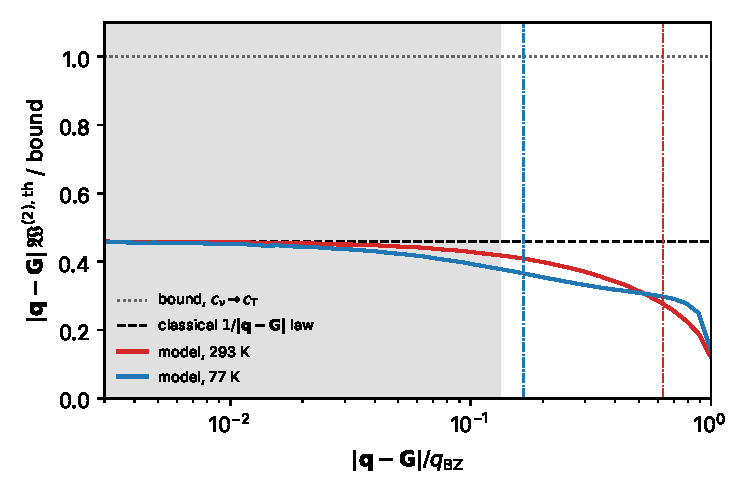
\includegraphics[width=\linewidth]{figures/ch11/limit11_3b.pdf}
\captionof{figure}{Thermal two-phonon weight times $|\vect{q} - \vect{G}|$, in units of the bound \cref{eq:11.3-tds} with $c_{\mathrm{min}}$ replaced by the transverse speed (dotted, one), for $\vect{G} = \vect{G}_{111}$ of silicon and $\vect{q} - \vect{G}$ parallel to $\vect{q}$, against $|\vect{q} - \vect{G}|/q_{\mathrm{BZ}}$. Model: isotropic elastic medium with the speeds $v_L = [(B + \frac43G)/\rho_T]^{1/2} = 8.95$ and $v_T = (G/\rho_T)^{1/2} = \SI{5.34}{km.s^{-1}}$ of silicon, with $G$ the Hill shear modulus, the mean of the Voigt value $G_{\mathrm{V}} = (C_{11} - C_{12} + 3C_{44})/5 = \SI{68.0}{GPa}$ and the Reuss value $G_{\mathrm{R}} = 5(C_{11} - C_{12})C_{44}/[4C_{44} + 3(C_{11} - C_{12})] = \SI{64.9}{GPa}$, exactly longitudinal and transverse polarizations, wavevectors cut at $|\vect{Q}| < q_{\mathrm{BZ}}$, and the full thermal factors $\coth(\omega_1/2T)\coth(\omega_2/2T) - 1$. Dashed: the classical $1/|\vect{q} - \vect{G}|$ law, 0.46 of the bound. Solid: the model at \SI{293}{K} (red) and \SI{77}{K} (blue). Dash-dotted: the boundary $|\vect{q} - \vect{G}| = T/c_{\mathrm{T}}$ of the classical soft pair at each temperature. Gray: within \SI{10}{\percent} of the classical law at \SI{293}{K}, $|\vect{q} - \vect{G}| \le 0.13\,q_{\mathrm{BZ}}$; at \SI{77}{K} the same holds below $0.065\,q_{\mathrm{BZ}}$. At \SI{10}{mK} the boundary lies at $2\times10^{-5}\,q_{\mathrm{BZ}}$.}\label{fig:11-limit-3b}
\par}
\smallskip
The law needs both phonons to be classical, $c_\nu|\vect{q} - \vect{G}| \ll T$. Farther from the peak the thermal occupations fall off and the weight drops below the law, and at the zone scale the dispersion and the regular two-phonon terms dominate.
\end{limitbox}

In a dark-matter detector the second-order thermal diffuse scattering is negligible. At \SI{10}{mK} the classical region ends at $|\vect{q} - \vect{G}| = T/c_{\mathrm{T}} = \SI{48}{meV}$, with the transverse speed $c_{\mathrm{T}}$ of \cref{lim:11.3b}, and the coefficient, which carries $T^2$, is $10^{-9}$ of its room-temperature value. The second-order term matters for the X-ray and neutron data, taken warm, that calibrate the lattice response, and for any rate quoted at \SI{77}{K} or above. At room temperature, a tenth of the zone momentum away from the (111) peak of silicon, the singular thermal weight is as large as the whole incoherent two-phonon weight there, 1.07 times it in the model of the limit check. A calculation at $T > 0$ evaluates the two-phonon coherence in reciprocal space and never as the real-space sum of \cref{eq:11.3-weight}.

\subsection{The charge vertex at large momentum}

For a coupling to charge, the dark photon of \cref{sec:11.2}, the electrons are part of the vertex, and $c_\kappa$ is no longer a number. Every result of this section assumed that $c_\kappa$ is a number; for a coupling to nucleons this assumption is exact, since the nucleons move with their nucleus. At momentum transfers small compared with the zone the electrons follow the nuclei adiabatically, and their effect is the Born effective charge and the screening of \cref{sec:11.2}. Far above the zone the question is how much of the electron cloud a displaced atom carries along, at the momentum transfer $q$ itself. A rigid neutral atom contributes $Z_\kappa - f_\kappa(q)$, with $f_\kappa$ the form factor of its electron cloud (\cref{sec:8.6}), and what the rigid atom misses is the deformation of the electron density as the atom moves. The deformation obeys one exact constraint. Summed over the atoms of a cell, for a displacement that is the same in every cell, the deformation is the change of the electron density under a uniform translation of the crystal. At the Fourier component $\vect{G}$ this change is $\ii G_\alpha$ times the density component itself, since with $n_e(\vect{q}) = \sum_j\ee^{\ii\vect{q}\cdot\vect{r}_j}$ a translation by $\vect{u}$ multiplies that component by $\ee^{\ii\vect{G}\cdot\vect{u}}$. The core shells follow their nucleus closely, polarized by the small residual field at the nucleus. The valence share is the open problem. It is not known how fast the deformation of the bonding charge decays between about 3 and \SI{20}{keV}: a calculation with pseudopotentials gives densities that are unphysical inside the core radius, above about \SI{10}{keV} in silicon, and a free-atom model has no bonds. The answer needs an all-electron calculation of displaced atoms in a large cell, with the translation sum rule as its test. Until that calculation is done, the multiphonon response of a charge coupling far above the zone rests on the rigid-atom vertex as an assumption, while that of a nucleon coupling does not.
